\documentclass[a4paper, twocolumn]{article}
\usepackage[pdftex, hidelinks]{hyperref}

\usepackage{bm}
\usepackage{xcolor}
\usepackage[T1]{fontenc}
\usepackage[utf8]{inputenc}
\usepackage{algorithmic}
\usepackage{algorithm}
\usepackage{amsfonts}
\usepackage{amssymb}
\usepackage{courier}
\usepackage{booktabs}
\usepackage{graphicx}
\usepackage{listings}
\usepackage{mathtools}
\usepackage{amssymb}
\lstset{basicstyle=\footnotesize\ttfamily,
breakatwhitespace = false,
breaklines = true,
keepspaces = true,
language = R,
showspaces = false,
showstringspaces = false,
belowcaptionskip = \bigskipamount,
framerule = 0.80pt,
frame = tb,
belowskip = \bigskipamount,
escapeinside={<@}{@>}}

\title{TDDE01 -- Machine Learning \\
Group 9 Laboration Report 6}
\author{{Martin Estgren \texttt{<mares480>}} \\
{Erik S. V. Jansson \texttt{<erija578>}} \\
{Sebastian Maghsoudi \texttt{<sebma654>}} \\~\\
{Linköping University (LiU), Sweden}}

\begin{document}
\pagenumbering{arabic}
    \maketitle % Generate.
    
    In this assignment we are tasked with approximating a sinus function using a neural net with one hidden layer of 10 nodes. The activation function we will use is the sigmoid function with batched gradient descent and resilient back propagation. 

    \lstinputlisting[firstline=7, lastline=9]{share/neuralnet.r}

    First a set of 50 randomly generated observations from the sinus function and split in two parts of equal size, one for training and one for validation. We create 10 neural nets, each with a different cut-off threshold for the gradient descent. We consider the thresholds 0.001, .... , 0.01 in steps of 0.001. 

    \lstinputlisting[firstline=18, lastline=20]{share/neuralnet.r}

    \begin{equation} \label{eq:sigmoid}
        \sigma(u) = \frac{1}{1 + e^{-u}}
    \end{equation}

    \begin{equation} \label{eq:batch_gradient}
        \bm{w}_{(i)} = \bm{w}_{(i-1)} - \eta_k \nabla E(\bm{w}_{(i-1)})
    \end{equation}

    \begin{equation} \label{eq:perceptron}
        \hat{y}_j(\bm{x}) = \sigma(w_0 + \sum_{h=1}^{H} \sigma(w_{0h} + \bm{w}_h^\intercal\bm{x}))
    \end{equation}

    \begin{enumerate}
        \item{\textbf{Sigmoid Activation Function:} ``S''-shaped function which converges $\sigma(u) = 1$ as $u \to \infty$ and $\sigma(u) = 0$ as $u \to -\infty$. Used in Equation~\ref{eq:perceptron}.}
        \item{\textbf{Batch Gradient Descent:} finds the ``step'' in the right direction for \emph{minimizing error} $E$. This is achieved with the \emph{gradient} of $E$ given in respect to the weights $\bm{w}$; giving a \emph{hyperplane}.}
        \item{\textbf{Single-Layer Neural Network Estimator:} uses Equations~\ref{eq:sigmoid} and \ref{eq:batch_gradient} to find $\hat{y}_j$ by finding the parameters $\bm{w}$ in each layer (a linear equation) by means of \emph{gradient descent} and producing a \emph{non-linear result in subsequent layers} by the \emph{activation function}. This is the primary reason why neural networks are so flexible \& general.}
    \end{enumerate}

    We calculate the S.S.E of each of the nets using the validation set and pick the one with the lowest error-rate. In the list below the S.S.E for each of the thresholds can be observed.

    \lstinputlisting[firstline=22, lastline=28]{share/neuralnet.r}

    \begin{table}[h!]
        \begin{center}
            \begin{tabular}{cc}
                \toprule
                \textbf{Threshold} & \textbf{S.S.E.} \\
                \midrule
                0.001 & 0.01367691527 \\
                0.002 & 0.01262419958 \\
                0.003 & 0.00988418900 \\
                0.004 & 0.00850089424 \\
                0.005 & 0.00955545744 \\
                0.006 & 0.00974372099 \\
                0.007 & 0.01583926857 \\
                0.008 & 0.01649252416 \\
                0.009 & 0.02112490377 \\
                0.010 & 0.02735909554 \\
                \bottomrule
            \end{tabular}
        \end{center}
        \caption{Neural Network Values}
        \label{tab:forecast}
    \end{table}
    The best threshold was observed to be 0.004.
    
    We recreate the neural net with the threshold 0.004 and generate predictions for the full data set of 50 observations. The result can be seen in figure~\ref{fig:predictions}.
    \begin{figure}[h!]
        \centering
        \caption{Neural Network}
        \label{fig:network}
        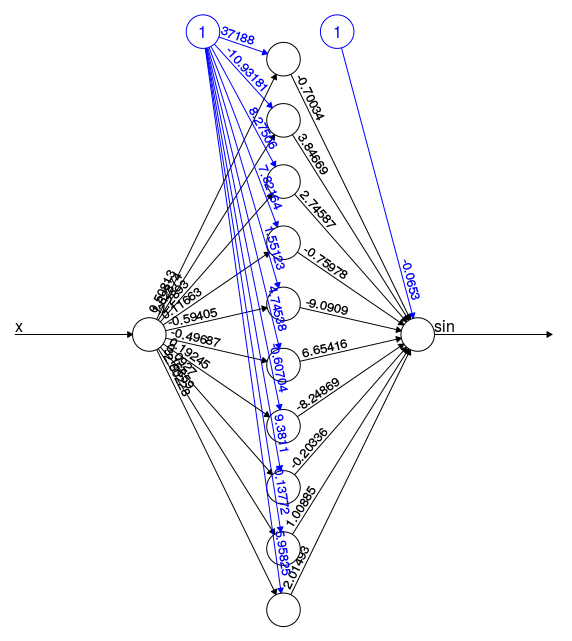
\includegraphics[width=0.46\textwidth]{share/network.png}
    \end{figure}
    The figure above shows a graph representation of the neural net. The black numbers are the individual weights and the blue ones are the intersections for each node.

    \begin{figure}[h!]
        \centering
        \caption{Neural Network's Produced Predictions (in the graph are \textcolor{blue}{raw values} and \textcolor{red}{predicted values}).}
        \label{fig:predictions}
        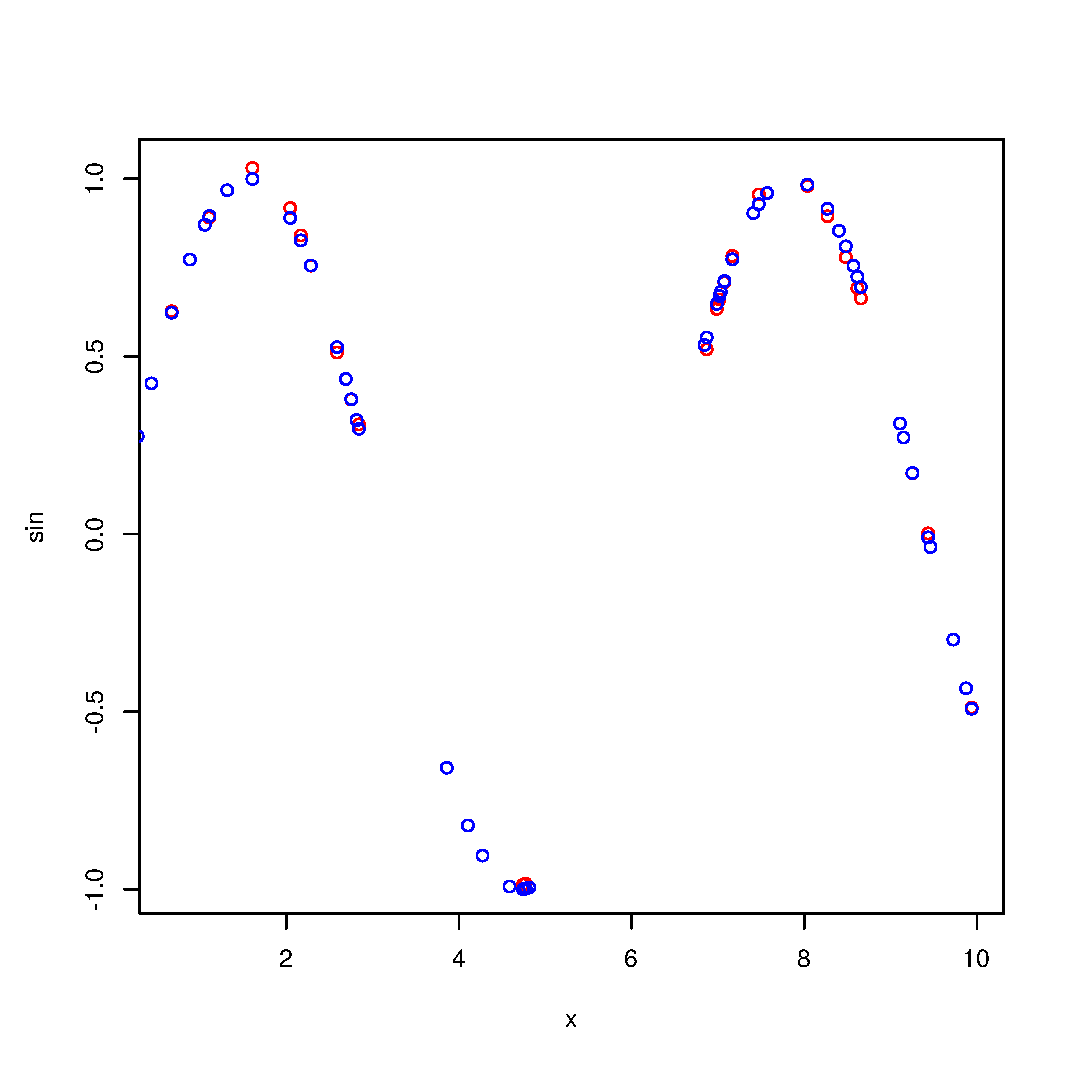
\includegraphics[width=0.5\textwidth]{share/predictions.eps}
    \end{figure}
    As we can observe in the figure above. The neural net produces a good estimate for the sinus function. Given the sample data.

    \section*{Contributions}

    This report was a joint effort between all group members, and as such, everyone has contributed equally.
    \begin{itemize}
        \item{\textbf{Martin Estgren:} all explanatory text in the report and most of the analysis.}
        \item{\textbf{Erik S. V. Jansson:} provided the listings and the figures.}
        \item{\textbf{Sebastian Maghsoudi:} in depth analysis of the report and results.}
    \end{itemize}

    \nocite{*} % No warnings.
    \bibliographystyle{alpha}
    \bibliography{report}
    \onecolumn \appendix
    \section*{Appendix}

    \lstinputlisting[caption={Feed-Forward Backpropagating Neural Network Sine Estimator Script}, label={lst:neuralnet}]{share/neuralnet.r}
    \lstinputlisting[caption={Output About the Produced Neural Network in the Assignment}, label={lst:properties}]{share/output.txt}

\end{document}
